\documentclass[12pt]{article}

\usepackage{tikz}
\usetikzlibrary{calc}
\usepackage[margin=1in]{geometry} 
\usepackage{amsmath,amsthm,amssymb}
\usepackage{tikz}
\usepackage{natbib}
\usepackage{subcaption}
\usepackage[utf8]{inputenc}
\usepackage{enumitem}
\usepackage{setspace}
\usepackage{color}
\usepackage{soul}
\newtheorem{definition}{Definition}
\newtheorem*{pf}{Proof}
\newtheorem{cl}{Claim}
\newtheorem{prop}{Proposition}
\newtheorem{thm}{Theorem}[section]
\newtheorem{cor}{Corollary}[section]
\newtheorem{axiom}{Axiom}[section]
\newtheorem{p}{Problem}[section]
\newtheorem{solution}{Solution}[section]
\usepackage{cancel}
\newtheorem{lem}{Lemma}[section]
\theoremstyle{definition}
\newtheorem{dfn}{Definition}[section]
\newtheorem{ex}{Example}[section]
\newtheorem{pb}{Problem}[section]
\newtheorem{obs}{Observation}[section]
 \newenvironment{s}{%\small%
        \begin{trivlist} \item \textbf{Solution}. }{%
            \hspace*{\fill} $\blacksquare$\end{trivlist}}%
\onehalfspacing
\usepackage{ragged2e}

\setlength{\parskip}{1em}
\title{On Graphical Methods in Stochastic Choice\footnote{I am thankful to Christopher Chambers and Yusufcan Masatlioglu for helpful discussions. I am particularly thankful to Peter Caradonna for fruitful conversations during which the idea behind this paper was developed.\\
Turansick:  Department of Economics, Georgetown University, ICC 580  37th and O Streets NW, Washington DC 20057.  E-mail:  \texttt{cmt152@georgetown.edu}}}

\author{Christopher Turansick}
\date{\today}

\begin{document}

\maketitle


\begin{abstract}
    In recent years there has been an influx of papers which use graph theoretic tools to study stochastic choice. \citet{fiorini2004short} serves as a base for this literature by providing a graphical representation of choice probabilities and showing that every interior node of this graph must satisfy inflow equals outflow. We show that this inflow equals outflow property is almost characteristic of choice probabilities. In doing so, we characterize choice probabilities through graph theoretic tools. As an application of this result, we provide a novel characterization of stochastic rationality on an incomplete domain.
\end{abstract}

\section{Introduction}

The stochastic choice paradigm is oft used to study the repeated choices of a single consumer as well as the aggregate choices of a population of consumers.
The literature on stochastic choice posits that the apparent randomness of choice arises due to multiple potential reasons including unobserved heterogeneity across agents and time, random attention, and a preference for variation. In recent years, there has been an influx of papers which use graph theoretic tools to study stochastic choice and specifically the random utility model of \citet{block1959random}. To our knowledge, \citet{fiorini2004short} is the first to bring graph theoretic tools to stochastic choice. Using these tools, \citet{fiorini2004short} offers a short proof of the characterization of random utility from \citet{falmagne1978representation}. One of the key insights of \cite{fiorini2004short} is that when choice probabilities are represented with a specific graph, this graph satisfies inflow equals outflow at each one of its interior nodes.

Our main result shows that this preservation of flow property is almost characteristic of choice probabilities. We show that a function satisfies inflow equals outflow at each interior node of the flow diagram, the graph from \citet{fiorini2004short}, if and only if it has a constant sum in each choice set, $\sum_{x \in A}f(x,A)=\sum_{y\in B}f(y,B)$. We are able to characterize choice probabilities as a corollary of this result with two more axioms. The first axiom asks that there is a total of one flow leaving the initial node of the flow diagram. This along with inflow equals outflow gives us that our function sums to one at every choice set. The second axiom asks that, at each node, the total flow associated with the choice $x$ from each weakly higher node must be non-negative. This axiom ensures that choice probabilities are non-negative.

In a recent paper, \citet{kono2023axiomatization} offers a characterization of random utility when every choice set is observed but the choice probabilities of some alternatives may be unobserved. This characterization requires one additional axiom beyond what \citet{falmagne1978representation} uses to characterize random utility. This new axiom is a statement about the (augmented) value of a cut of their graphical representation. A cut is bipartition of the set of nodes of a graph. Call these two sets of nodes $S$ and $T$. The augmented value of a cut is the total flow from $S$ to $T$ minus the total flow from $T$ to $S$. \citet{kono2023axiomatization} asks that every cut have a non-negative augmented value. This result motivates the second part of our main result. We show that a function has a constant sum in each choice set if and only if every cut of its flow diagram has the same augmented value.

As an application of our main result, we offer a new characterization of random utility for incomplete data sets. The classic characterization of random utility for incomplete data sets is from \citet{mcfadden1990stochastic}. Their method asks that there is some probability distribution over preferences which induce the observed choice probabilities. One way to get their axiom is to look at the alternative linear program of this existence question. One problem with this method is that it produces an axiom that references the underlying representation. An alternative way of posing the stochastic rationality question is by asking if there is an extension of the observed choice probabilities to a complete domain which satisfy the conditions of \citet{falmagne1978representation}. Initially, this method may appear to give messy conditions as asking for an extension of choice probabilities is a statement about probabilities and asking that they satisfy the conditions of \citet{falmagne1978representation} is a statement about the M\"{o}bius inverse of probabilities. Our main insight is that you can write the extension problem using only the M\"{o}bius inverse of choice probabilities using the flow conditions from our main result. Similar to \citet{mcfadden1990stochastic}, we then get our axiom by looking at the alternative linear program of the restatement of the stochastically rational extension linear program.

The rest of this paper is organized as follows. In Section 2, we introduce our mathematical and graphical preliminaries. In Section 3, we present our main result. In Section 4, we apply our main result to the random utility model. In Section 5, we conclude with a discussion and a review of the related literature.


\section{Preliminaries}
Let $X$ be a finite set of alternatives with typical elements $x$. Let $\mathcal{L}(X)$ be the set of linear orders of $X$ with typical element $\succ$. Let $\Delta(\mathcal{L}(X))$ be the set of probability distributions over $\mathcal{L}(X)$ with typical element $\nu$. Let $\mathcal{X}$ be a collection of nonempty subsets of $X$ with typical element $A$. Note that $\mathcal{X}$ need not be $2^X \setminus\{\emptyset\}$, the collection of \textit{all} nonempty subsets of $X$. Let $M(\succ,A)$ denote the element $x \in A$ such that $x \succ A \setminus\{x\}$. Let $N(x,A)=\{\succ|x \succ A \setminus \{x\}\}$ be the set of linear orders which are maximized by $x$ in $A$.

We are interested in functions $f:X \times 2^X\setminus\{\emptyset\} \rightarrow \mathbb{R}$ and the behavior of $f(x,A)$ when $x \in A$. Specifically, we are interested in characterizing set constant functions.

\begin{dfn}
    A function $f:X \times 2^X\setminus\{\emptyset\} \rightarrow \mathbb{R}$ is \textbf{set constant} if for each $A,B \in 2^X\setminus\{\emptyset\}$, $\sum_{x \in A}f(x,A) = \sum_{y\in B}f(y,B)$.
\end{dfn}

Within the class of set constant functions, our goal is to develop a better understanding of random choice rules.

\begin{dfn}
A function $p:X \times 2^X\setminus\{\emptyset\} \rightarrow \mathbb{R}$ is called a \textbf{signed random choice rule} if $\sum_{x\in A} p(x,A)=1$. It is called a \textbf{random choice rule} if it is a signed random choice rule and $p(x,A)\geq 0$ for all $x \in A$.
\end{dfn}

Random choice rules capture the choice probabilities of a given alternative $x$ in choice set $A$. In order to study random choice rules, we utilize their M\"{o}bius inverse.

\begin{dfn}
    The \textbf{M\"{o}bius inverse} of a function $f:X \times 2^X\setminus\{\emptyset\} \rightarrow \mathbb{R}$ is given by the function $g:X \times 2^X\setminus\{\emptyset\} \rightarrow \mathbb{R}$ which is recursively defined as follows.\footnote{In the case of set inclusion, as we face here, the M\"{o}bius inverse can be defined explicitly as $g(x,A)=\sum_{A \subseteq B}(-1)^{|B\setminus A|}f(x,B)$.}
    \begin{equation*}
        f(x,A) = \sum_{A \subseteq B} g(x,B)
    \end{equation*}
\end{dfn}

\citet{rota1964foundations} studies M\"{o}bius inversion and shows that the M\"{o}bius inverse is always well-defined, each function $f$ has a unique M\"{o}bius inverse $g$, and each M\"{o}bius inverse $g$ has a unique generating function $f$.

\subsection{Graphical Construction and Concepts}
In this section we introduce our main graphical construction, first introduced by \citet{fiorini2004short} to study random utility, as well as the concepts we use to analyze this construction. Given a finite set of alternatives $X$ and a function $f:X \times 2^X\setminus\{\emptyset\} \rightarrow \mathbb{R}$, we construct the \textbf{flow diagram} associated with $f$ as follows. The nodes of the flow diagram are indexed by the elements of $2^X$, the power set of $X$. We use the set indexing a node to refer to that node. There exists an edge between two nodes $A$ and $B$ if one of the following is true.
\begin{enumerate}
    \item $A \subseteq B$ and $|B \setminus A| = 1$
    \item $B \subseteq A$ and $|A \setminus B| = 1$
\end{enumerate}
In other words, the edge set of this graph is formed by applying the covering relation of $\subseteq$ to $X$. For the edge connecting $A$ and $A \setminus \{x\}$, we assign $g(x,A)$, the M\"{o}bius inverse of $f$, as its edge weight. Figure \ref{fig:flowdiagram} presents the flow diagram given a set $X = \{a,b,c\}$ and a function $f$ with M\"{o}bius inverse $g$.

\begin{figure}
    \centering
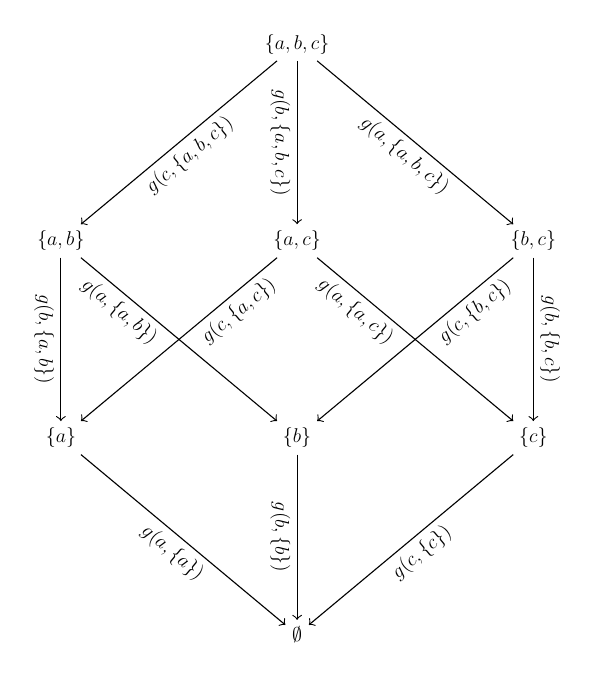
\begin{tikzpicture}[scale=.5, transform shape]
    \Large
    \tikzstyle{every node} = [rectangle]
    
    %level 0
        \node (a) at (6,0) {$\emptyset$};
        
    %level 1
        \node (b) at (0,5) {$\{a\}$};
        \node (c) at (6,5) {$\{b\}$};
        \node (d) at (12,5) {$\{c\}$};
        
    %level 2
        \node (e) at (0,10) {$\{a,b\} $};
        \node (f) at (6,10) {$\{a,c\}$};
        \node (g) at (12,10) {$\{b,c\}$};

    %level 3
        \node (h) at (6,15) {$\{a,b,c\}$};
        
    %edges
        \draw [->] (h) -- (f) node[midway, below, sloped] {$g(b,\{a,b,c\})$};
        \draw [->] (h) -- (g) node[midway, below, sloped] {$g(a,\{a,b,c\})$};  
        \draw [->] (h) -- (e) node[midway, below, sloped] {$g(c,\{a,b,c\})$}; 

        
        \draw [->] (e) -- (b) node[midway, below, sloped] {$g(b,\{a,b\})$}; 
        \draw [->] (e) -- (c) node[pos=.25, below, sloped] {$g(a,\{a,b\})$};
        \draw [->] (f) -- (b) node[pos=.25, below, sloped] {$g(c,\{a,c\})$};
        \draw [->] (f) -- (d) node[pos=.25, below, sloped] {$g(a,\{a,c\})$};
        \draw [->] (g) -- (c) node[pos=.25, below, sloped] {$g(c,\{b,c\})$};
        \draw [->] (g) -- (d) node[midway, above, sloped] {$g(b,\{b,c\})$}; 

        \draw [->] (b) -- (a) node[midway, below, sloped] {$g(a,\{a\})$};
        \draw [->] (c) -- (a) node[midway, below, sloped] {$g(b,\{b\})$};
        \draw [->] (d) -- (a) node[midway, below, sloped] {$g(c,\{c\})$};
    
    \end{tikzpicture}
    \caption{The flow diagram for the set $X = \{a,b,c\}$ and function $f$ with M\"{o}bius inverse $g$.}
    \label{fig:flowdiagram}
\end{figure}

Given our flow diagram, we can consider paths on this flow diagram.

\begin{dfn}
    Given a flow diagram for $X$ and $f$, a \textbf{path} is a collection of nodes $\{A_1, \dots, A_n\}$ such that $A_1 =X$, $A_n=\emptyset$, $n= |X|+1$, and $i > j \implies A_i \subsetneq A_j$. We use the shorthand $\pi$ to refer to an arbitrary path whose nodes we do not specify.
\end{dfn}

We use $\Pi_X$ to denote the set of paths for the flow diagram of $X$ and $f$. Further, we let $E_X$, with typical element $e$, denote the set of edges of the flow diagram for $X$ and $f$. We say that a path $\pi$ passes through an edge $e$ if $e$ connects nodes $A$ and $A \setminus \{x\}$ and $A,A\setminus\{x\} \in \pi$.

\begin{dfn}
    Given the flow diagram of a set $X$ and a function $f$, a \textbf{flow assignment} is a function $r:\Pi_X \rightarrow \mathbb{R}$ such that for each edge $e$ we have $\sum_{\pi \in \Pi_X} r(\pi) \mathbf{1}\{\pi \text{ passes through } e\} \leq g(x,A)$ where $g(x,A)$ is the edge weight of $e$.
\end{dfn}

We say that the value $u$ of a flow assignment $r$ is given by $u(r)=\sum_{\pi \in \Pi_X}r(\pi)$. The value of a flow assignment captures the total flow assigned to all paths. There is a connection between the feasible flow assignments of a graph and cuts of a graph.

\begin{dfn}
    Given a flow diagram, a \textbf{cut} $C$ of the flow diagram is a bipartition of the set of nodes of the flow diagram with each set in the bipartition being nonempty. A \textbf{sink-source cut} is a cut such that $X$ and $\emptyset$ are in different sets of the bipartition.
\end{dfn}

\begin{figure}
    \centering
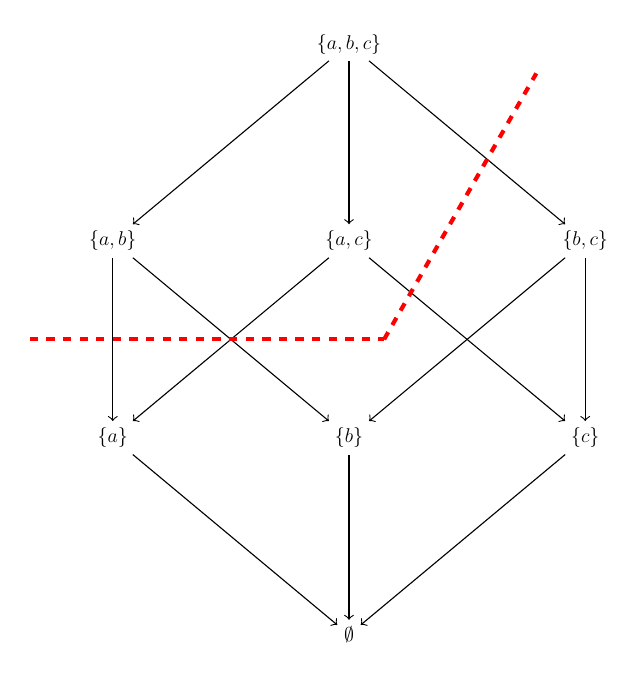
\begin{tikzpicture}[scale=.5, transform shape]
    \Large
    \tikzstyle{every node} = [rectangle]
    
    %level 0
        \node (a) at (6,0) {$\emptyset$};
        
    %level 1
        \node (b) at (0,5) {$\{a\}$};
        \node (c) at (6,5) {$\{b\}$};
        \node (d) at (12,5) {$\{c\}$};
        
    %level 2
        \node (e) at (0,10) {$\{a,b\} $};
        \node (f) at (6,10) {$\{a,c\}$};
        \node (g) at (12,10) {$\{b,c\}$};

    %level 3
        \node (h) at (6,15) {$\{a,b,c\}$};
        
    %edges
        \draw [->] (h) -- (f) node[midway, below, sloped] {};
        \draw [->] (h) -- (g) node[midway, below, sloped] {};  
        \draw [->] (h) -- (e) node[midway, below, sloped] {}; 

        
        \draw [->] (e) -- (b) node[midway, below, sloped] {}; 
        \draw [->] (e) -- (c) node[pos=.25, below, sloped] {};
        \draw [->] (f) -- (b) node[pos=.25, below, sloped] {};
        \draw [->] (f) -- (d) node[pos=.25, below, sloped] {};
        \draw [->] (g) -- (c) node[pos=.25, below, sloped] {};
        \draw [->] (g) -- (d) node[midway, above, sloped] {}; 

        \draw [->] (b) -- (a) node[midway, below, sloped] {};
        \draw [->] (c) -- (a) node[midway, below, sloped] {};
        \draw [->] (d) -- (a) node[midway, below, sloped] {};

        \draw[dashed, red, line width=1.5pt] ([xshift=-60pt]$ (e)!0.5!(b) $ ) --  ([xshift=-60pt]$ (g)!0.5!(c) $ );
        \draw[dashed, red, line width=1.5pt] ([xshift=-60pt]$ (g)!0.5!(c) $ ) --  ([xshift=50pt, yshift=50pt]$ (g)!0.5!(h) $ );
    
    \end{tikzpicture}
    \caption{Above, the red dashed line represents the cut of the flow diagram. In this case, $\{\{a,b,c\}, \{a,b\},\{a,c\}\}$ and $\{\{b,c\}, \{a\}, \{b\}, \{c\}, \emptyset\}$ are the two sets which partition $2^X$, the set of nodes of the flow diagram.}
    \label{fig:cut}
\end{figure}


From here on out, whenever we use cut we refer specifically to sink-source cuts. Figure \ref{fig:cut} gives an example of a cut of a flow diagram where $X = \{a,b,c\}$. We let $\mathcal{C}_X$ denote the collection of cuts the flow diagram associated with $X$ and $f$. Given a cut $C$, we use $S$ to refer to the set in the cut bipartition which contains $X$ and $T$ to refer to the set in the cut bipartition which contains $\emptyset$. 
The value $v$ of a cut $C$ is the sum of edge weights across edges connecting sets in different sets of the cut bipartition.
    \begin{equation*}
        v(C) = \sum_{A \in 2^X\setminus \{\emptyset\}} \sum_{x \in A} g(x,A) \mathbf{1}\{(A \in S \wedge A \setminus \{x\} \in T) \vee (A \in T \wedge A \setminus \{x\} \in S)\}
    \end{equation*}

To calculate the value of the cut in Figure \ref{fig:cut}, we would just sum the edge weights of the edges which intersect with the dashed red line. Given a graph with non-negative edge weights, \citet{ford1956maximal} shows that the minimum value of a cut of a graph is equal to the maximum value of a flow assignment to that graph.\footnote{Theorem 3 of \citet{dogan2022every} provides a similar result which allows edge weights to be negative. However, this result is not sufficient for our analysis.} We need a slightly non-standard definition of the value of a cut as we work with potentially negative edge weights.

\begin{dfn}
    Given a cut $C$, the \textbf{augmented value} $w$ of the cut is given by the following.
    \begin{equation}
        w(C) = \sum_{A \in 2^X\setminus \{\emptyset\}} \sum_{x \in A} g(x,A)(\mathbf{1}\{A \in S \wedge A \setminus \{x\} \in T\} - \mathbf{1}\{A \in T \wedge A \setminus \{x\} \in S\})
    \end{equation}
\end{dfn}

While the value of a cut rewards an edge for going from $S$ to $T$ and for going from $T$ to $S$, the augmented value of a cut rewards an edge for going from $S$ to $T$ but punishes an edge for going from $T$ to $S$. Consider a cut and a path. This path could in theory pass between $S$ and $T$ multiple times and thus be counted multiple times in the value of the cut. By considering the augmented value of a cut, we are able to deal with this double counting of paths.


\section{Main Result}
In this section we present our main result, a characterization of set constant functions through their M\"{o}bius inverse. We then provide further conditions on the M\"{o}bius inverse to ensure that a function is a signed random choice rule and then a random choice rule. Our first axiom is called inflow equals outflow.

\begin{axiom}
A function $f:X \times 2^X\setminus\{\emptyset\} \rightarrow \mathbb{R}$ with M\"{o}bius inverse $g$ satisfies \textbf{inflow equals outflow} if the following holds for all $A \in 2^X \setminus \{X,\emptyset\}$.
\begin{equation}
    \sum_{x \in A}g(x,A) = \sum_{y \not \in A}g(y,A \cup \{y\})
\end{equation}
\end{axiom}

As a necessary step in characterizing random utility via the M\"{o}bius inverse of choice probabilities, \citet{falmagne1978representation} shows that every random choice rule satisfies inflow equals outflow. While presenting a graphical proof Falmagne's result, \citet{fiorini2004short} shows that inflow equals outflow can be interpreted as inflow equaling outflow at every node of the flow diagram which is neither $X$ nor $\emptyset$. Part of our contribution is showing that inflow equals outflow almost characterizes random choice rules. Our second axiom leverages cuts and their augmented values.

\begin{axiom}
    A function $f:X \times 2^X\setminus\{\emptyset\} \rightarrow \mathbb{R}$ satisfies \textbf{constant cuts} if the flow diagram of $X$ and $f$ satisfies $\max_{C \in \mathcal{C}_X}w(C) = \min_{C \in \mathcal{C}_X} w(C)$.
\end{axiom}

In the previous section, we noted that our focus on augmented weights is in order to avoid double counting of paths. The constant cuts axiom is exactly asking that no matter how you count paths via a cut and sum across their corresponding edge weights, as long as there is no double counting, the total sum of edge weights will be constant.

\begin{thm}\label{maintheorem}
Consider a function $f:X \times 2^X\setminus\{\emptyset\} \rightarrow \mathbb{R}$. The following are equivalent.
\begin{enumerate}
    \item $f$ is set constant.
    \item $f$ satisfies inflow equals outflow.
    \item $f$ satisfies constant cuts.
\end{enumerate}
\end{thm}

While we relegate the proof to the appendix, we present a sketch of the proof here. The equivalence of $f$ being set constant and $f$ satisfying inflow equals outflow comes from the following equation.

\begin{equation}\label{inflowandconstant}
    \sum_{x \in A}g(x,A) - \sum_{y \in X\setminus A}g(y,A \cup \{y\}) = \sum_{x \in A}f(x,A) - \sum_{y \in X}f(y,X)
\end{equation}

We begin by showing that this is the case when $A = X \setminus \{y\}$ which relies on the observation that the M\"{o}bius inverse of $f$ is equal to $f$ when evaluated at $X$. In other words, we have $g(x,X)=f(x,X)$. If we recall the definition of the M\"{o}bius inverse, it is immediate that the left hand side of Equation \ref{inflowandconstant} reduces to the right hand side. In this case, it immediately follows that inflow equals outflow is equivalent to $f$ being set constant. The rest of proving this equivalence relies on inductively showing that Equation \ref{inflowandconstant} holds for other choices of $A$ when either inflow equals outflow or set constant holds.

In the next part of the proof we show that inflow equals outflow is equivalent to constant cuts. To show that inflow equals outflow implies constant cuts, we show that, when inflow equals outflow holds, you can always completely decompose the flow diagram into a flow assignment. By this, we mean that you can always find a flow assignment which assigns flow at an edge equal to the edge weight of that edge. We call such a flow assignment a flow decomposition. This means that we can calculate the edge weights of any edge by calculating the flow through that edge from a flow decomposition. We then consider any cut of the flow diagram. Since the augmented value of a cut counts every path at least once and avoids double counting of paths and using the fact that we can calculate an edge weight from flows through that edge, the augmented value of any cut is equal to the value of a flow decomposition. Since the total flow of a flow decomposition is constant, this gives us constant cuts.

To show that constant cuts implies inflow equals outflow, we consider two specific cuts. The first cut we consider is given by $S=\{A \subseteq X|n\leq |A| \}$ and the second cut we consider is $S' = \{A \subseteq X|n \leq |A|\} \setminus B$ where $|B|=n$. When calculating the augmented values of these two cuts, each edge leaving $B$ is counted for $S$ but not for $S'$ and each edge going into $B$ is counted for $S'$ but not for $S$. This means that the difference between the augmented value of these two cuts is given by $\sum_{x \in A}g(x,B) - \sum_{y \in X\setminus A}g(y,B \cup \{y\})$. Since $f$ satisfies constant cuts, this difference is zero and thus $f$ satisfies inflow equals outflow.

As is clear from our proof of Theorem \ref{maintheorem}, we do not need to consider every cut in order to show that constant cuts implies inflow equals outflow. We can ease the computational burden of checking constant cuts by considering a subclass of cuts.

\begin{dfn}
    A cut $C=(S,T)$ is \textbf{single-crossing} if for every path $\{A_i\}_{i=1}^n$, $i>j$ and $A_j \in T$ imply $A_i \in T$.
\end{dfn}

Single-crossing cuts are exactly the cuts which guarantee there is no double counting of paths. As an immediate corollary of our proof, it is sufficient to check every single-crossing cut in order to show that constant cuts holds.

\begin{cor}\label{singlecrossingcor}
    Let $\mathcal{C}_X^{SC}$ be the set of single-crossing cuts of the flow diagram of $X$ and $f$. $f$ satisfies constant cuts if and only if $\max_{C \in \mathcal{C}_X^{SC}}w(C) = \min_{C \in \mathcal{C}_X^{SC}} w(C)$. Further, this is equivalent to $\max_{C \in \mathcal{C}_X^{SC}}v(C) = \min_{C \in \mathcal{C}_X^{SC}} v(C)$.
\end{cor}

The second part of Corollary \ref{singlecrossingcor} makes the observation that if no path travels between $S$ and $T$ multiple times, then it is not necessary to use the augmented weight to deal with double counting. By characterizing set constant functions, we have done most of the work involved with characterizing random choice rules in terms of their M\"{o}bius inverse. All that is left to do is to ensure that our function $f$ sums to one in each set and is non-negative everywhere. The following corollaries of Theorem \ref{maintheorem} capture these conditions.

\begin{cor}\label{srcr}
    Let $f$ be a set constant function with M\"{o}bius inverse $g$. $f$ is a signed random choice rule if and only if $\sum_{x \in X}g(x,X)=1$.
\end{cor}

Corollary \ref{srcr} says that if we have a set constant function, all we need to do to get a signed random choice rule is to guarantee that our function sums to one on some set, in this case $X$.

\begin{cor}\label{rcr}
    Let $f$ be a signed random choice rule with M\"{o}bius inverse $g$. $f$ is a random choice rule if and only if for each nonempty $A \subseteq X$ and $x \in A$, we have $\sum_{A \subseteq B}g(x,B) \geq 0$.
\end{cor}

The condition in Corollary \ref{rcr} is a direct translation of the non-negativity condition of probabilities into their M\"{o}bius inverse. Taken together, Theorem \ref{maintheorem} and Corollaries \ref{srcr} and \ref{rcr} fully characterize random choice rules. Our key axiom in this characterization is inflow equals outflow. This axiom captures the preservation of flow at each node in the flow diagram which is neither $X$ nor $\emptyset$. This property is equivalent to the preservation of choice probabilities at each choice set. The equivalence between preservation of flow and the preservation of choice probabilities is exactly why the flow diagram is a natural representation of choice probabilities.

\section{An Application to Random Utility}
In this section we use Theorem \ref{maintheorem} to provide a new characterization of stochastic rationality. We consider random choice rules on a potentially limited domain.

\begin{dfn}
    A random choice rule $p:X \times \mathcal{X} \rightarrow \mathbb{R}$ is \textbf{stochastically rational} if there exists some probability distribution over linear orders, $\nu \in \mathcal{L}(X)$, such that for each $A \in \mathcal{X}$ and $x \in A$ we have the following.
    \begin{equation*}
        p(x,A) = \sum_{\succ \in \mathcal{L}(X)}\nu(\succ)\mathbf{1}\{x \succ A \setminus \{x\}\}
    \end{equation*}
\end{dfn}

We use $q$ to denote the M\"{o}bius inverse of a random choice rule $p$. \citet{falmagne1978representation} was the first to characterize stochastically rational random choice rules and did so through the use of the Block-Marschak polynomials \citep{block1959random}. The Block-Marschak polynomials are exactly the M\"{o}bius inverse of a random choice rule.

\begin{thm}[\citet{falmagne1978representation}]\label{falmagne}
    A random choice rule $p:X \times 2^X\setminus\{\emptyset\} \rightarrow \mathbb{R}$ with M\"{o}bius inverse $q$ is stochastically rational if and only if $q(x,A)\geq 0$ for every nonempty $A \subseteq X$ and $x \in A$.
\end{thm}

Theorem \ref{falmagne} is appealing in many ways, one of which is that it characterizes stochastic rationality with a finite set of linear inequalities. However, one of the shortcomings of the characterization is that it relies on the observation of choice probabilities on \textit{every} nonempty subset of $X$. This is generally an overly restrictive assumption on data. \citet{mcfadden1990stochastic} offer an alternative approach to characterizing stochastic rationality which weakens the full domain assumption.

\begin{thm}[\citet{mcfadden1990stochastic}]\label{mcfadden}
    A random choice rule $p:X \times \mathcal{X} \rightarrow \mathbb{R}$ is stochastically rational if and only if for any finite sequence $\{(x_i,A_i)\}_{i=1}^n$ with $x_i \in A_i \in \mathcal{X}$ the following holds.
    \begin{equation*}
        \sum_{i=1}^np(x_i,A_i) \leq \max_{\succ \in \mathcal{L}(X)}\sum_{i=1}^n \mathbf{1}\{x_i \succ A_i \setminus \{x_i\}\}
    \end{equation*}
\end{thm}

Theorem \ref{mcfadden} solves the complete domain problem but requires an infinite number of linear inequalities and its statement requires a reference to the underlying representation. Our upcoming characterization combines the characterization of \citet{falmagne1978representation} with the insight from our Theorem \ref{maintheorem} in order to pose the stochastic rationality question for arbitrary domains without referencing the underlying representation. Our characterization relies on two supplemental functions.

\begin{dfn}
    A function $c:2^X \rightarrow \mathbb{R}$ is a \textbf{capacity} if $c(\emptyset)=0$.
\end{dfn}

\begin{dfn}
    A function $a:X\times \mathcal{X} \rightarrow \mathbb{R}$ is an \textbf{assignment}.
\end{dfn}

In order to best interpret the role of capacities and assignments, we introduce the following definition.

\begin{dfn}
    An assignment and capacity pair $(a,c)$ is \textbf{feasible} if the follow inequality holds.
    \begin{equation}\label{feasible}
        \sum_{A \in \mathcal{X}}\sum_{x \in A}p(x,A)a(x,A) \leq c(X)
    \end{equation}
\end{dfn}

The role of an assignment $a$ is to assign some weight to the event that $x$ is chosen from $A$. When combined with the probability that $x$ is chosen from $A$, $p(x,A)$, this weight is given by $a(x,A)p(x,A)$. Each set $A$ has a capacity $c(A)$ which must contain the total weight of the events where $x$ is chosen from $B$ for each $B \subseteq A$. Feasibility simply asks that the total weight put on choosing some element from some set is less than the capacity of $X$, the total capacity of our environment. Our characterization relies on a second type of feasibility.

\begin{dfn}
    An assignment and capacity pair $(a,c)$ is \textbf{locally feasible} if for each $(x,A)$ with  $x \in A \in 2^X \setminus \{\emptyset\}$ the following inequality holds.
    \begin{equation}\label{localfeas}
        \sum_{x \in B \in \mathcal{X}, B \subseteq A} a(x,B) \leq c(A) - c(A \setminus \{x\}) 
    \end{equation}
\end{dfn}

Local feasibility is local in two senses. It is local in that it captures the change in capacity between two sets $A$ and $A\setminus \{x\}$ and in that it captures feasibility along one path of the flow diagram. In order to better understand this connection, we must first interpret the paths of the flow diagram in terms of linear orders. A path $\{X,X\setminus \{x_1\},\dots,\{x_n\}\}$ on the flow diagram corresponds to the linear order $x_1 \succ \dots \succ x_n$. Figure \ref{fig:pathtopref} gives an example of a path and its corresponding linear order. To better understand this bijective relationship between paths and linear orders, we turn to a result of \citet{falmagne1978representation}.

\begin{thm}[\citet{falmagne1978representation}]\label{rumidentification}
    A distribution over linear orders $\nu$ is a random utility representation of a random choice rule $p:X \times 2^X \setminus \{\emptyset\} \rightarrow \mathbb{R}$ if and only if the following holds for all nonempty $A \subseteq X$ and $x \in A$.
    \begin{equation*}
        q(x,A) = \sum_{\succ \in \mathcal{L}(X)}\nu(\succ)\mathbf{1}\{X\setminus A \succ x \succ A\setminus \{x\}\}
    \end{equation*}
\end{thm}

Theorem \ref{rumidentification} says that a random utility representation of a random choice rule must put probability weight on linear orders which choose $x$ from $A$ but not from any $A \cup \{y\}$ equal to $q(x,A)$, the M\"{o}bius inverse of $p(x,\cdot)$ evaluated at $A$. Recall that our flow diagram assigns $q(x,A)$ as the edge weight for the edge connecting nodes $A$ and $A \setminus \{x\}$. This means that the edge weight of the edge connecting $A$ and $A\setminus \{x\}$ corresponds to the event in which a preference which chooses $x$ from $A$ but not from any $A \cup \{y\}$ is drawn. If we take the intersection of these events along a full path, then the unique preference in the intersection of these events is the linear order associated with that path.

\begin{figure}
    \centering
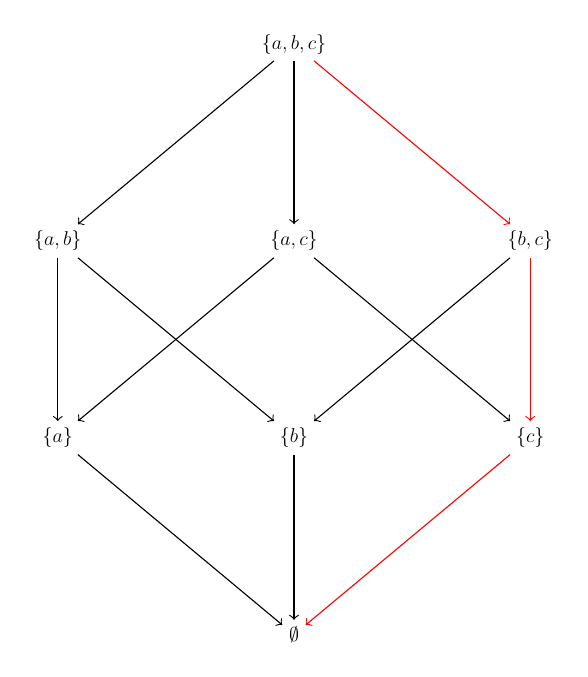
\begin{tikzpicture}[scale=.5, transform shape]
    \Large
    \tikzstyle{every node} = [rectangle]
    
    %level 0
        \node (a) at (6,0) {$\emptyset$};
        
    %level 1
        \node (b) at (0,5) {$\{a\}$};
        \node (c) at (6,5) {$\{b\}$};
        \node (d) at (12,5) {$\{c\}$};
        
    %level 2
        \node (e) at (0,10) {$\{a,b\} $};
        \node (f) at (6,10) {$\{a,c\}$};
        \node (g) at (12,10) {$\{b,c\}$};

    %level 3
        \node (h) at (6,15) {$\{a,b,c\}$};
        
    %edges
        \draw [->] (h) -- (f) node[midway, below, sloped] {};
        \draw [->, red] (h) -- (g) node[midway, below, sloped] {};  
        \draw [->] (h) -- (e) node[midway, below, sloped] {}; 

        
        \draw [->] (e) -- (b) node[midway, below, sloped] {}; 
        \draw [->] (e) -- (c) node[pos=.25, below, sloped] {};
        \draw [->] (f) -- (b) node[pos=.25, below, sloped] {};
        \draw [->] (f) -- (d) node[pos=.25, below, sloped] {};
        \draw [->] (g) -- (c) node[pos=.25, below, sloped] {};
        \draw [->, red] (g) -- (d) node[midway, above, sloped] {}; 

        \draw [->] (b) -- (a) node[midway, below, sloped] {};
        \draw [->] (c) -- (a) node[midway, below, sloped] {};
        \draw [->, red] (d) -- (a) node[midway, below, sloped] {};

        %\draw[dashed, red, line width=1.5pt] ([xshift=-60pt]$ (e)!0.5!(b) $ ) --  ([xshift=-60pt]$ (g)!0.5!(c) $ );
        %\draw[dashed, red, line width=1.5pt] ([xshift=-60pt]$ (g)!0.5!(c) $ ) --  ([xshift=50pt, yshift=50pt]$ (g)!0.5!(h) $ );
    
    \end{tikzpicture}
    \caption{Above, the red path $\{\{a,b,c\},\{b,c\},\{c\},\emptyset\}$ corresponds to the linear order $a \succ b \succ c$.}
    \label{fig:pathtopref}
\end{figure}

We now return to the interpretation of local stability. If we first start at the empty set and then follow some path up to $X$, local stability gives us a sequence of inequalities.
\begin{equation}\label{locallist}
    \begin{split}
        &a(x_n,\{x_n\}) \leq c(\{x_n\}) - 0 \\
        &a(x_{n-1},\{x_n,x_{n-1}\}) + a(x_{n-1},\{x_{n-1}\}) \leq c(\{x_n,x_{n-1}\})-c(\{x_n\}) \\
        %&a(x_{n-2},\{x_n,x_{n-1},x_{n-2}\}) + a(x_{n-2},x_{n-1},x_{n-2}\}) + a(x_{n-2},\{x_{n-2}\}) \leq c(\{x_n,x_{n-1},x_{n-2}\}) -c(\{x_n,x_{n-1}\})\\
        &\dots
    \end{split}
\end{equation}

If we sum across this entire sequence, we are left with the following inequality.

\begin{equation}\label{determsum}
    \sum_{x_i \in X} \sum_{x_i \in A , \forall j<i, x_j \not \in A}a(x_i,A) \leq c(X)
\end{equation}

Equations \ref{feasible} and \ref{determsum} are connected when we consider the case of classically rational choices. To see this observe the following.

\begin{obs}\label{iia}
    A random choice rule $p:X \times 2^X \setminus \{\emptyset\} \rightarrow \mathbb{R}$ can be written as $p(x,A)=\mathbf{1}\{x \succ A \setminus x\}$ for some $\succ \in \mathcal{L}(X)$ if and only if for each $x \in X$, $p(x,A)=\mathbf{1}\{A \subseteq B_x\}$ for some $B_x \in 2^X \setminus \{\emptyset\}$.
\end{obs}

Observation \ref{iia} just restates the classic result that the independence of irrelevant alternative condition (see \citet{chernoff1954rational}, \citet{arrow1959rational}, and \citet{sen1971choice}) is equivalent to classic rationality. The thing to note is that when independence of irrelevant alternative is translated into choice probabilities, it states that each element's choice probabilities should be a step function. By applying Observation \ref{iia} to Equation \ref{feasible}, thus imposing classic rationality on our random choice rule, Equation \ref{feasible} exactly reduces to Equation \ref{determsum}. In this sense, local feasibility reduces to feasibility for every classically rational choice function.

Local feasibility is a local constraint in a second way. In Equation \ref{locallist}, we chose to sum across every element of the list. If instead, we sum across the first $n$ elements of the list and let $A = \bigcup_{i=1}^n \{x_i\}$, we are left with the following inequality.

\begin{equation}\label{subdsum}
    \sum_{x_i \in A} \sum_{x_i \in B , \forall j<i, x_j \not \in B}a(x_i,B) \leq c(A)
\end{equation}

Equation \ref{subdsum} is exactly Equation \ref{determsum} restricted to the subdomain of $A$. Now suppose that we want to verify that this inequality holds for $A \cup \{x_{n+1}\}$. Further, suppose that we do not know whether Equation \ref{subdsum} holds with equality. Local feasibility is exactly the necessary and sufficient condition needed to verify that Equation \ref{subdsum} holds for $A \cup \{x_{n+1}\}$. Thus our local feasibility condition is a statement about local conditions that imply feasibility when choices are classically rational.

From our prior discussion, it should be clear that there is some connection between local feasibility and feasibility for stochastically rational random choice rules. This connection follows straight from the classically rational case. A stochastically rational random choice rule can be written as a convex combination of classically rational random choice rules. Given a preference $\succ$, we can consider the path corresponding to $\succ$ and its induced Equation \ref{determsum}. This preference has some probability weight on it in the random utility representation $\nu$. If we sum across each variant of Equation \ref{determsum}, assigning each of these different variants weight equal to $\nu(\succ)$, the probability weight of the linear order that generated this variant, then the inequality we are left with is exactly the feasibility condition of Equation \ref{feasible}. This leads us to our characterization.

\begin{thm}\label{rumme}
    A random choice rule $p:X \times \mathcal{X} \rightarrow \mathbb{R}$ is stochastically rational if and only if every locally feasible assignment and capacity pair $(a,c)$ is also feasible.
\end{thm}

Our main innovation over Theorem \ref{mcfadden} is that we use Theorem \ref{maintheorem} to rewrite the stochastic rationality linear program without reference to any preferences. One way to interpret the condition in Theorem \ref{mcfadden} is to first write down a linear program $rM=p$ where $M$ is a matrix that encodes the choices of each linear order, $p$ encodes the observed choice probabilities, and $r$ encodes a potential probability distribution over linear orders. The condition in Theorem \ref{mcfadden} is then related to the alternative linear program through Farkas's Lemma (see \citet{border2007introductory} and \citet{borderAlternative}) We rewrite the stochastic rationality linear program as follows.
\begin{align}\label{linearpro}
    \left[\begin{array}{c}
        D\\
        \hline
        E\\
        \hline
        F
    \end{array}\right] q = \left[\begin{array}{c}
        P \\
        \hline
        \mathbf{0} \\
        \hline
        1
    \end{array}\right] \nonumber
    \\
    q \geq 0
\end{align}

In Equation \ref{linearpro}, we use $q$ to represent the M\"{o}bius inverse of a potential full domain random choice rule. $Dq=P$ encodes that this potential full domain random choice rule must agree with our observed random choice rule on observed choice sets. We use $Eq=0$ to encode the inflow equals outflow axiom and use $Fq=1$ to encode that $\sum_{x\in X}q(x,X)=1$. From Theorem \ref{falmagne}, we know that a full domain random choice rule is stochastically rational if and only if the M\"{o}bius inverse of choice probabilities is non-negative. This condition implies $\sum_{A\subseteq B}q(x,B)\geq 0$, the condition from Corollary \ref{rcr}. This means that the condition $q \geq 0$ encodes both stochastic rationality as well as the last condition necessary to ensure that the potential $q$ is in fact the M\"{o}bius inverse of some full domain random choice rule. We can now obtain the alternative linear program through Farkas's Lemma and some minor manipulation leaves us with our condition in Theorem \ref{rumme}.

\section{Discussion}

In this paper, we argue that the M\"{o}bius inverse of choice probabilities as well graph theoretic tools are well suited for studying stochastic choice. In doing so, we show that random choice rules are characterized by three properties of their M\"{o}bius inverse, with inflow equals outflow being the defining axiom. While we do not claim that these tools are the best tools for every stochastic choice problem, they provide an alternative perspective and a means by which to study the stochastic choice paradigm. As an example, consider the classic model of \citet{luce1959individual}.

\begin{dfn}
    A random choice rule $p:X \times 2^X \setminus \{\emptyset\}$ is \textbf{consistent} with the Luce model if there exists a function $h:X \rightarrow \mathbb{R}^{++}$ such that $p(x,A)=\frac{h(x)}{\sum_{y\in A}h(y)}$.
\end{dfn}

It is well known that the Luce model is characterized by positive choice probabilities and the stochastic independence of irrelevant alternatives condition. We can reinterpret these conditions with our set of tools to get the following result.

\begin{thm}\label{luce}
    Consider a random choice rule $p:X \times 2^X \rightarrow \mathbb{R}$ with M\"{o}bius inverse $q$. The following are equivalent.
    \begin{enumerate}
        \item $p$ is consistent with the Luce model.
        \item $p(x,A)>0$ for all $x \in A \subseteq X$ and $\frac{p(x,A)}{p(y,A)}=\frac{p(x,B)}{p(y,B)}$ for all $x,y \in A \cap B$.
        \item $q(x,A)>0$ for all $x \in A \subseteq X$ and $\frac{q(x,A)}{q(y,A)}=\frac{q(x,B)}{q(y,B)}$ for all $x,y \in A \cap B$.
    \end{enumerate}
\end{thm}

The equivalence of the first two conditions is the result of \citet{luce1959individual}. The equivalence with the third condition is novel and tells us that choice probabilities having a constant ratio across sets is equivalent to a constant proportional assignment of inflows to outflows at each node in our flow diagram.

We also apply our characterization of random choice rules to offer a new characterization of stochastic rationality. In a recent paper, \citet{gonczarowski2019infinity} shows that Theorem \ref{mcfadden} can be extended to allow for infinite $X$. While our Theorem \ref{rumme} is focused on finite $X$, it can be extended using the same tools as \citet{gonczarowski2019infinity}. The condition that \citet{gonczarowski2019infinity} asks for is that the condition in Theorem \ref{mcfadden} must hold for every finite sequence of $(x_i,A_i)$. This is equivalent to the condition from Theorem \ref{mcfadden} holding on every finite subdomain of their potentially infinite collection of choice sets. Since Theorem \ref{mcfadden} and our Theorem \ref{rumme} both characterize stochastic rationality for finite $X$, it follows that this is equivalent to the condition from our Theorem \ref{rumme} holding for every finite subdomain.

Finally, we note that the graphical methods we develop in this paper may offer computational improvements over current methods. \citet{kitamura2018nonparametric} develops a hypothesis test for stochastic rationality and \citet{smeulders2021nonparametric} shows that this test is NP-hard. A large part of this computation complexity is due to the fact that this test involves calculating the matrix $M$ which encodes the choice of every linear order at every (observed) choice set. When choices are observed at every choice set, this $M$ matrix has one row for each path of the flow diagram. Alternatively, a matrix which encodes our local stability condition need only have as many rows as there are edges in the flow diagram, which is strictly less than the number of paths in the flow diagram when $|X|\geq 5$.\footnote{To see this, note that the number of paths in the flow diagram is equal to the number of linear orders of $X$, which is given by $|X|!$ where $!$ denotes factorial. On the other hand, the number of edges in the flow diagram is equal to the number of edges leaving a node summed over each node. This is given by $\sum_{i=1}^{|X|} i \binom{|X|}{i}$ where $\binom{|X|}{i}$ represents the binomial coefficient.} As such, there may be ways to leverage our Theorem \ref{rumme} in order to reduce the computational burden of testing for stochastic rationality.

\subsection{Related Literature}
Our paper is related to two strands of literature. The first strand applies graphical methods to study questions in the stochastic choice paradigm. To our knowledge, \citet{fiorini2004short} is the first to bring graph theoretic tools to the study of stochastic choice. \citet{fiorini2004short} studies the characterization of random utility presented in \citet{falmagne1978representation} and provides a novel proof which leverages the observation that choice probabilities satisfy inflow equals outflow and that this can be naturally represented on the flow diagram. More recently, \citet{davis2018extended} studies the flow polytopes of other random utility style models including models of random weak orders, interval orders, and semiorders. \citet{doignon2022adjacencies} studies the adjacency of vertices in the linear order polytope and its associated flow polytope, our flow diagram. \citet{chang2022approximating} uses the adjacency of linear orders in order to study when random-coefficient models can approximate random utility models. \citet{turansick2022identification} uses the flow diagram to study the uniqueness properties of the random utility model. \citet{dogan2022every} provides an extension of the result of \citet{ford1956maximal} in order to show that every random choice rule can be represented as a linear combination of linear orders. \citet{saito2017axiomatizations} and \citet{chambers2021correlated} provide alternate proofs of this result with the latter using a flow decomposition argument similar to the one used in the proof of our Theorem \ref{maintheorem}. Further, \citet{chambers2021correlated} extends the flow diagram to allow for choice with multiple dimension in order to study which random joint choice rules have well defined marginal choice probabilities. \citet{sprumont2022regular} uses flows to study which binary choice probabilities admit an extension to the full domain while maintaining monotonicity of choice probabilities. Finally, as mentioned prior, \citet{kono2023axiomatization} uses a graphical construction as well as flows and cuts in order to characterize random utility when the choice probabilities of some alternatives are unobserved.

The second strand of literature that our paper contributes to is the one which offers characterizations of the random utility model. \citet{falmagne1978representation} is the first to characterize the random utility and does so by asking that the M\"{o}bius inverse of choice probabilities be non-negative. \citet{monderer1992stochastic} provides an alternate proof of this result using methods from cooperative game theory. \citet{cohen1980random} considers an extension of the result of \citet{falmagne1978representation} to an infinite domain. \citet{nandeibam2009probabilistic} provides a different characterization of random utility using positive linear functionals. \citet{mcfadden1990stochastic} offers a characterization of random utility when the choice domain is incomplete. \citet{stoye2019revealed} offers a short proof of this result using tools from convex analysis. \citet{mcfadden2005revealed} offers an extension of this result to an infinite domain under some regularity conditions. Recently, \citet{gonczarowski2019infinity} extends this result to an infinite domain without any regularity conditions. \citet{clark1996random} offers an alternative characterization of random utility in the case of an incomplete domain using DeFinetti's coherency axiom. 

\appendix

\section{Proofs}

\subsection{Proof of Theorem \ref{maintheorem}}

We begin by showing the equivalence of $f$ satisfying inflow equals outflow and $f$ being set constant. We begin with the necessity of inflow equals outflow. Consider a function $f$ with M\"{o}bius inverse $g$ such that $f$ is set constant. We proceed via induction on the size of the complement of $A$. For the base case, let $A=X\setminus\{x\}$. Observe that $f(x,X)=g(x,X)$ We have the following.

\begin{equation*}
    \begin{split}
        \sum_{x \in X A}g(x,A) & = \sum_{x \in A} f(x,A)-g(x,X) \\
        & =\sum_{x\in X}f(x,X) -\sum_{x \in A}f(x,X) \\
        & = f(x,X) =g(x,X)
    \end{split}
\end{equation*}

Above, the first equality holds by the definition of M\"{o}bius inverse. The second equality holds from $f$ being set constant. The third equality follows after collecting like terms. This shows that the base case of inflow equals outflow holds. Now assume that inflow equals outflow holds for all $B$ with $|X \setminus B| < n$. Let $A$ be such that $|X \setminus A|=n$.

\begin{equation*}
    \begin{split}
        \sum_{x \in A} g(x,A) & = \sum_{x\in A}f(x,A) - \sum_{x\in A} \sum_{A \subsetneq A'}g(x,A') \\
        & = \sum_{x\in A}f(x,A) - \sum_{A \subsetneq A'}[\sum_{x\in A'}g(x,A') - \sum_{x\in A' \setminus A}g(x,A')] \\
        & = \sum_{A \subsetneq A'} \sum_{x \in A' \setminus A}g(x,A') - \sum_{A \subsetneq A' \subsetneq X} \sum_{x \in A'} g(x,A') \\
        & = \sum_{A \subsetneq A'} \sum_{x \in A' \setminus A}g(x,A') - \sum_{A \subsetneq A' \subsetneq X} \sum_{y \in X \setminus A'}g(y,A \cup \{y\}) \\
        & = \sum_{z \in X \setminus A} g(z,A \cup\{z\})
    \end{split}
\end{equation*}

Above, the first equality holds by the definition of M\"{o}bius inverse. The second equality just adds zero. The third equality holds as $g(x,X)=f(x,X)$ and because $f$ is set constant. The fourth equality holds by the induction hypothesis. The fifth equality follows from combining like terms. Thus the above string of equalities show that inflow equals outflow is necessary. We now show sufficiency. Now suppose $f$ satisfies inflow equals outflow. Consider some $A \subsetneq X$.

\begin{equation*}
    \begin{split}
        \sum_{x \in A} g(x,A) & = \sum_{x\in A}[f(x,A) - \sum_{A \subsetneq A'}g(x,A')] \\
        & = \sum_{x\in A}f(x,A) - \sum_{A \subsetneq A'}[\sum_{x\in A'}g(x,A') - \sum_{x\in A' \setminus A}g(x,A')] \\
        & =[\sum_{x\in A}f(x,A)-\sum_{x\in X}f(x,X)] + \sum_{A \subsetneq A'} \sum_{x \in A' \setminus A}g(x,A') - \sum_{A \subsetneq A' \subsetneq X} \sum_{x \in A'} g(x,A') \\
        & =[\sum_{x\in A}f(x,A)-\sum_{x\in X}f(x,X)] +  \sum_{A \subsetneq A'} \sum_{x \in A' \setminus A}g(x,A') - \sum_{A \subsetneq A' \subsetneq X} \sum_{y \in X \setminus A'}g(y,A \cup \{y\}) \\
        & =[\sum_{x\in A}f(x,A)-\sum_{x\in X}f(x,X)] +  \sum_{z \in X \setminus A} g(z,A \cup\{z\})
    \end{split}
\end{equation*}
The first equality above holds due to the definition of M\"{o}bius inverse. The second equality just adds zero. The third equality holds as $f(x,X)=g(x,X)$. The fourth equality holds by inflow equals outflow. The fifth equality follows from combining like terms. By inflow equals outflow, we know that $\sum_{x\in A}g(x,A)=\sum_{z \in X \setminus A}g(z,A\cup\{z\})$. This means that the above string of equalities gives us that $\sum_{x\in A}f(x,A)=\sum_{x\in X}f(x,X)$. Since $A$ is arbitrary, this tells us that $f$ is set constant.

We now show the equivalence between $f$ satisfying inflow equals outflow and $f$ satisfying constant cuts. Consider a function $f$ which satisfies inflow equals outflow and has M\"{o}bius inverse $g$. We now show that it satisfies constant cuts. Consider the flow diagram of $f$. We now construct a flow decomposition. Let $s$ be a function from the set of paths of the flow diagram to $\mathbb{R}$.
    \begin{enumerate}
        \item Initialize at $i=0$. For each path $\rho$, set $s(\rho)=0$.
        \item Choose an edge $e_i$ such that its edge weight is the minimal among all edges with non-zero edge weight. If the edge weight of $e_i < 0$ proceed to step 3. If $e_i>0$ proceed to step 4. If there is no non-zero edge weight, terminate the algorithm.
        \item $e_i$ is a part of some path $\rho_i$. Set $s(\rho_i)=s(\rho_i)+w(e_i)$. For each edge $e'$ on path $\rho_i$, set the edge weight of $e'$ equal to $w(e')-w(e_i)$. Return to step $2$.
        \item The minimal edge weight among non-zero edge weights is positive. As the flow diagram satisfies inflow equals outflow at every stage of the algorithm (see below), this means that $e_i$ is an edge of some path $\rho_i$ such that every edge of $\rho_i$ has a strictly positive edge weight. Set $s(\rho_i)=s(\rho_i)+w(e_i)$. For each edge $e'$ on path $\rho_i$, set the edge weight of $e'$ equal to $w(e')-w(e_i)$. Return to step $2$.
    \end{enumerate}
    
    We now argue that this algorithm terminates and terminates with each edge weight being equal to zero. This algorithm only adds or subtracts edge weight along a full path. This means that inflow equals outflow is preserved at each step of the algorithm. Further, in step $4$, since $w(e_i)$ is minimal among non-zero edge weights, the edge weights of all edges along $\rho_i$ are non-negative with $w(e_i)$ being equal to zero at the end of step $4$. So, repeated iterations of step $3$ takes every edge weight and makes them non-negative. Then, repeated iterations of step $4$ take non-negative edge weights and make them zero. Consider the augmented value of any cut $C=(S,T)$. Every path starts at $X$ and ends at $\emptyset$. This means that every path starts in $S$ and ends in $T$. Further, if a path leaves $S$ and goes to $T$, it must return to $S$ from $T$ before it can leave $S$ and go to $T$ again. This means that a path will always leave $S$ one more time than it leaves $T$. Let $P$ be the set of paths of the flow diagram.

    \begin{equation*}
        \begin{split}
                    w(C) & = \sum_{A \in 2^X\setminus \{\emptyset\}} \sum_{x \in A} g(x,A)(\mathbf{1}\{A \in S \wedge A \setminus \{x\} \in T\} - \mathbf{1}\{A \in T \wedge A \setminus \{x\} \in S\}) \\
                    & = \sum_{\rho \in P}s(\rho)
        \end{split}
    \end{equation*}

    Above, the first inequality follows from the definition of augmented value of a cut. The second equality holds due to the logic of the prior paragraph and because the algorithm which generated $s$ leaves zero flow everywhere on the flow diagram. In simpler terms, the total flow assigned to any edge is equal to the edge weight of that edge. Since $C$ was an arbitrary cut, constant cuts holds.

    Now suppose that constant cuts holds. Consider the cuts. $C$ is defined by $S=\{A \subseteq X|n\leq |A| \}$ and $C'$ is defined by $S' = \{A \subseteq X|n \leq |A|\} \setminus B$ where $|B|=n$ and $0 < n < |X|$. By construction, the only edges which $C$ counts that $C'$ does not count are the edges leaving $B$. Similarly, the only edges which $C'$ counts but $C$ does not count are the edges which enter into $B$. This gives us the following.

    \begin{equation*}
        \begin{split}
            w(C) - w(C') & = \sum_{x \in B} g(x,A) - \sum_{y \not \in B}g(y,B \cup\{y\}) \\
            & = 0
        \end{split}
    \end{equation*}

    Above, the first equality follows from collecting like terms. The second equality follows from constant cuts. Thus constant cuts implies inflow equals outflow and we are done.

    \subsection{Proof of Corollary \ref{singlecrossingcor}}
    As inflow equals outflow implies constant cuts, inflow equals outflow also implies constant single-crossing cuts. Now observe that the two cuts used to show constant cuts implies inflow equals outflow are single-crossing cuts. This means that constant single-crossing cuts implies inflow equals outflow. Now observe that in single-crossing cuts, no path travels from $T$ to $S$. This means that the weight and augmented weight of single-crossing cuts coincide.

    \subsection{Proof of Corollary \ref{srcr}}
    Let $f$ with M\"{o}bius inverse $g$ be set constant. As $\sum_{x \in X}g(x,X)=\sum_{x\in X}f(x,X)$ by the definition of the M\"{o}bius inverse, it immediately follows that a set constant $f$ is a signed random choice rule if and only if $\sum_{x \in X}g(x,X)=1$.

    \subsection{Proof of Corollary \ref{rcr}}
    Let $f$ with M\"{o}bius inverse $g$ be a signed random choice rule. Recall the definition of the M\"{o}bius inverse.
    \begin{equation*}
        f(x,A)=\sum_{A \subseteq B}g(x,B)
    \end{equation*}
    It then immediately follows that $f$ is a random choice rule if and only if $\sum_{A \subseteq B}g(x,B) \geq 0$ for all such $x \in B \subseteq X$.

    \subsection{Proof of Theorem \ref{rumme}}
    Let $N(x,A) = \{\succ \in \mathcal{L}(X)|x \succ A \setminus \{x\}\}$. A random choice rule on $X$ is stochastically rational if and only if there exists $\nu\in \Delta(\mathcal{L}(X))$ such that $p(x,A)=\sum_{\succ \in N(x,A)}\nu(\succ)$ for all $x\in A \in \mathcal{X}$. This is equivalent to the existence of such a $\nu$ and the existence of choice probabilities $p(y,B)$ for each $B \in (2^X \setminus\{\emptyset\})\setminus \mathcal{X}$ such that $p(x,A)=\sum_{\succ \in N(x,A)}\nu(\succ)$ for all $x\in A \in 2^X \setminus\{\emptyset\}$. By Theorem \ref{falmagne}, this is equivalent to the existence of choice probabilities $p(y,B)$ for each $B \in (2^X \setminus\{\emptyset\})\setminus \mathcal{X}$ such that $q(x,A)\geq 0$ for each $x \in A \in 2^X \setminus\{\emptyset\}$. By Theorem \ref{maintheorem}, this is equivalent to the existence of $q(x,A)\geq 0$ for each $x \in A \in 2^X \setminus\{\emptyset\}$ such that $q$ satisfies inflow equals outflow, the conditions of Corollary \ref{srcr} and Corollary \ref{rcr}, and $\sum_{A \leq C}q(x,C)=p(x,A)$ for all $x \in A \in \mathcal{X}$. Note that $q(x,A)\geq 0$ implies the condition of Corollary \ref{rcr}, $\sum_{A \leq B}q(x,B)=p(x,A)$ implies that the choice probabilities induced by $q$ agree with our observed choice probabilities, and $q(x,A) \geq 0$ implies that the induced choice probabilities are rationalizable by random utility.

    We now construct the matrix form of this linear program. Consider a matrix $D$ whose columns are indexed by $(x,A)$ for each $A \in 2^X \setminus\{\emptyset\}$ and each $x \in A$ and whose rows are indexed by $(y,B)$ for each $B \in \mathcal{X}$ and $y \in B$. The entry $d_{(y,B),(x,A)}=1$ if $B \subseteq A$ and $x=y$ and is equal to zero otherwise. $D$ encodes that our unobserved $q$ function must induce our observed choice probabilities. Let $P$ be a column vector indexed by $(y,B)$ for each $B \in \mathcal{X}$ and $y \in B$. Entry $p_{(y,B)}$ is equal to $p(y,B)$. Consider a matrix $E$ whose columns are indexed by $(x,A)$ for each $A \in 2^X \setminus\{\emptyset\}$ and each $x \in A$ and whose rows are indexed by $B \in 2^X \setminus\{X,\emptyset\}$. The entry $e_{B,(x,A)}$ is given as follows.
    \begin{equation*}
        e_{B,(x,A)}=\begin{cases} 1 & \text{ if } x \not \in B, A = B \cup \{x\} \\
        -1 & \text{ if } x \in B, A = B \\
        0 & \text{ otherwise}
        \end{cases}
    \end{equation*}
    $E$ encodes that our unobserved $q$ satisfy inflow equals outflow. Consider a row vector $F$ whose elements are indexed by $(x,A)$ for each $A \in 2^X \setminus\{\emptyset\}$ and each $x \in A$. The element $f_{(x,A)}$ is equal to one if $A=X$ and equal to zero otherwise. $F$ encodes that our unobserved $q$ satisfy $\sum_{x\in X}q(x,X)$. To be stochastically rational, we must impose $q \geq 0$ which implies the condition of Corollary \ref{rcr}. Thus the linear program we have constructed looks as follows.
    \begin{align}
        \left[\begin{array}{c}
        D\\
        \hline
        E\\
        \hline
        F
        \end{array}\right] q = \left[\begin{array}{c}
        P \\
        \hline
        \mathbf{0} \\
        \hline
        1
        \end{array}\right]
        \\
        q \geq 0
    \end{align}
    By Farkas's Lemma, (see Theorem 34 in \citet{borderAlternative} for a reference), there exists a solution to this linear program if and only if there does not exist a solution $r \in \mathbb{R}^M$ to the following linear program.
\begin{align}
    r^T\left[\begin{array}{c}
        D\\
        \hline
        E\\
        \hline
        F
    \end{array}\right] \leq 0 \\
    \left[\begin{array}{c|c|c}
        P & \mathbf{0} & 1
    \end{array}\right]\cdot r^T > 0
\end{align}
Writing out Equation $(13)$ gives us the following.
\begin{equation}
    \sum_{(y,B):y\in B \in \mathcal{X}} r(y,B)p(y,B) + r(X) > 0
\end{equation}
Above, $r(X)$ is the element of $r$ which is associated with the vector $F$. As $r(X)$ can be any real number, we can rewrite Equation $(14)$ as follows.
\begin{equation}
    \sum_{(y,B):y\in B \in \mathcal{X}} r(y,B)p(y,B) - r(X) > 0
\end{equation}
For a given $(x,A)$, Equation $(12)$ can be written as follows.
\begin{equation}
    \sum_{B:x \in B \subseteq A, B \in \mathcal{X}} r(x,B) + r(A \setminus \{x\}) - r(A) \leq 0
\end{equation}
Above, in the case that $A \setminus \{x\} = \emptyset$, we define $r(\emptyset)=0$. Further, $r(X)$ shows up as $-r(X)$ as a consequence of our transformation of Equation $(14)$ into Equation $(15)$. The negation of the existence of some $r$ solving Equations $(15)$ and $(16)$ is equivalent to the negation of every locally feasible assignment and capacity pair $(a,c)$ being feasible. Thus it follows that the condition of Theorem \ref{rumme} holds if and only if $p$ is stochastically rational.

\subsection{Proof of Theorem of \ref{luce}}
The equivalence between the first two conditions was shown by \citet{luce1959individual}. We now show the equivalence between the third condition and the other two conditions. Suppose that $p$ is consistent with the Luce model. Then there exists weights $h(\cdot)$ such that $p(x,A) = \frac{h(x)}{\sum_{y\in A}h(y)}$. We will use the notation $h(A)$ to denote $\sum_{y\in A}h(y)$. Consider the following.
    \begin{equation*}
    \begin{split}
        q(x,A) & = \sum_{A \subseteq B} (-1)^{|B \setminus A|} p(x,B) \\
        & = \sum_{A \subseteq B} (-1)^{|B \setminus A|} \frac{h(x)}{h(B)} \\
        & =  h(x) \sum_{A \subseteq B} (-1)^{|B \setminus A|} \frac{1}{h(B)}
    \end{split}
\end{equation*}
Let $q(A,A) = \sum_{x \in A} q(x,A)$. Observe the following.
\begin{equation*}
    \begin{split}
        q(A,A) & = \sum_{x \in A} q(x,A) \\
        & = \sum_{x \in A}  h(x) \sum_{A \subseteq B} (-1)^{|B \setminus A|} \frac{1}{h(B)} \\
        & = h(A) \sum_{A \subseteq B} (-1)^{|B \setminus A|} \frac{1}{h(B)}
    \end{split}
\end{equation*}
Theorem 3.1 tells us that $q(A,A) = \sum_{y \in X \setminus A} q(y,A \cup \{y\})$. Observe the following.
\begin{equation*}
    q(x,A)=\frac{h(x)}{h(A)}q(A,A)
\end{equation*}
This gives us the following.
\begin{equation*}
    \begin{split}
        q(x,A) & = \frac{h(x)}{h(A)}q(A,A) \\
        & = \frac{h(x)}{h(A)}\sum_{y \in X \setminus A} q(y,A \cup \{y\}) \\
        & = \frac{h(x)}{h(A)}\sum_{y \in X \setminus A} \frac{h(y)}{h(A \cup \{y\})}q(A \cup \{y\},A \cup \{y\})
    \end{split}
\end{equation*}
The second equality above follows from inflow equals outflow. We can repeatedly apply the substitution shown on the second line above to the third line above. Since $q(X,X)=1$ and $X$ is finite, repeated applications of this substitution will leave us with an equation that is a sum and product of weights, $h(\cdot)$. Since each $h(x)$ is strictly positive, so too must be a sum and product of these weights. This gives us $q(x,A) >0$ for all $x \in A \subseteq X$. Observe the following.
\begin{equation*}
    \begin{split}
        \frac{q(x,A)}{q(y,A)} & = \frac{\sum_{A \subseteq B} (-1)^{|B \setminus A|} p(x,B)}{\sum_{A \subseteq B} (-1)^{|B \setminus A|} p(y,B)} \\
        & = \frac{\sum_{A \subseteq B} (-1)^{|B \setminus A|} p(x,B)}{(p(y,X)/p(x,X))\sum_{A \subseteq B} (-1)^{|B \setminus A|} p(x,B)} \\
        & = \frac{p(x,X)}{p(y,X)} \\
        & = \frac{q(x,X)}{q(y,X)}
    \end{split}
\end{equation*}
Above, the first equality follows from the definition of $q$. The second equality holds from the second condition of Theorem \ref{luce} The third equality follows from canceling like terms. The fourth equality holds due to the definition of $q$. This shows that the third condition of Theorem \ref{luce} is necessary. We now show sufficiency. Assume the third condition of Theorem \ref{luce} holds. Recall that $p(x,A) =\sum_{A \subseteq B}q(x,B)$. Thus if $q(x,B) >0$ for all $(x,B)$, it then follows that $p(x,A)>0$ for all $(x,A)$. Observe the following.
\begin{equation*}
    \begin{split}
        \frac{p(x,A)}{p(y,A)} & = \frac{\sum_{A \subseteq B} q(x,B)}{\sum_{A \subseteq B}q(y,B)} \\
        & = \frac{\sum_{A \subseteq B} q(x,B)}{(q(y,X)/q(x,X))\sum_{A \subseteq B}q(x,B)} \\
        & = \frac{q(x,X)}{q(y,X)} \\
        & = \frac{p(x,X)}{p(y,X)}        
    \end{split}
\end{equation*}
Above, the first equality holds by the definition of $q$. The second equality holds due to the third condition of Theorem \ref{luce}. The third equality follows from collecting like terms. The last equality holds from the definition of $q$. This shows that $p$ is consistent with the Luce model, so we are done.

\bibliographystyle{ecta}
\bibliography{graph}

\end{document}